\section{Contenedor con SGDB MySQL}

\subsection{Descripción}

Contenedor docker partiendo de una instalación base de MySQL, permitiendo consultas desde el exterior del contenedor.

\subsection{Archivo Dockerfile}

\begin{figure}[H]\center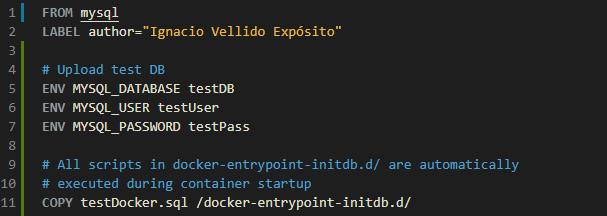
\includegraphics[width=.95\linewidth]{img/sgbd/s3.png}\caption{}\end{figure}

Creamos en el archivo Dockerfile un usuario para realizar las pruebas e incluímos una base de datos a partir de un script.

\subsection{Proceso de construcción}

\subsubsection{En local}

\begin{figure}[H]\center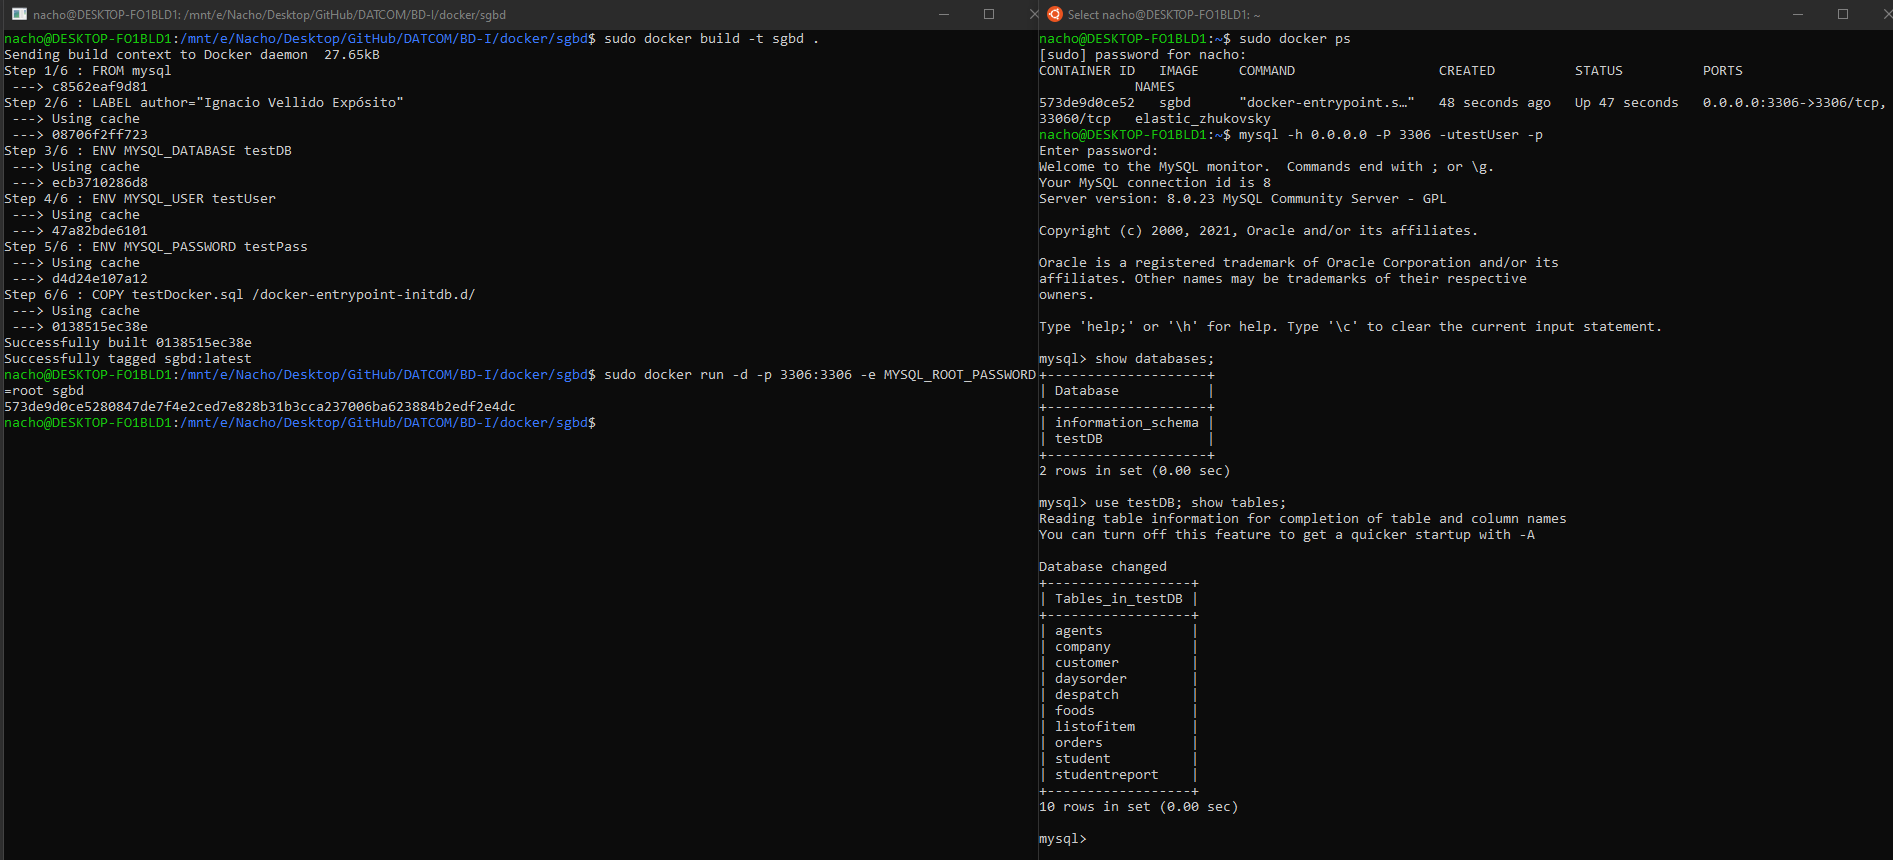
\includegraphics[width=.99\linewidth]{img/sgbd/s2.png}\caption{Construcción del contenedor y ejecución desde fuera de él.}\end{figure}

\begin{figure}[H]\center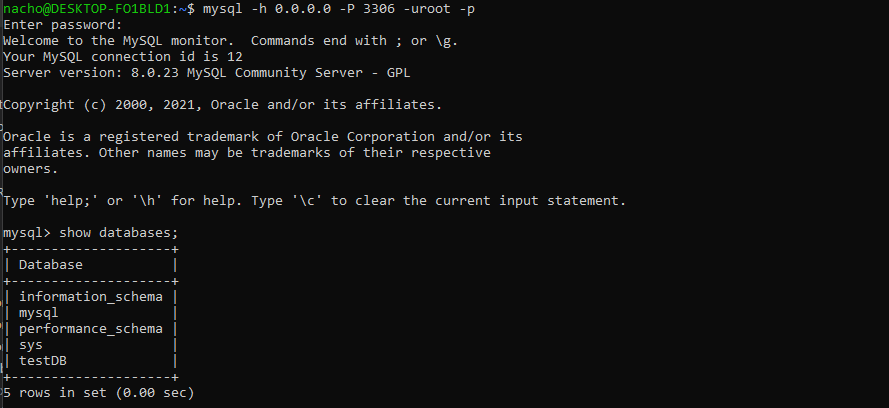
\includegraphics[width=.95\linewidth]{img/sgbd/s1.png}\caption{Entrando como usuario root.}\end{figure}

\subsubsection{En Azure}

Una vez más para desplegar el contenedor en Azure subimos la imágen al repositorio y creamos una nueva ``container instance''.

\vspace{\baselineskip}

Para este contenedor es necesario indicarle a Azure el puerto exportado en la imagen, y modificar el Dockerfile para incluir la contraseña del root (puesto que no se le puede indicar a Azure en el momento de ejecución).

\begin{figure}[H]\center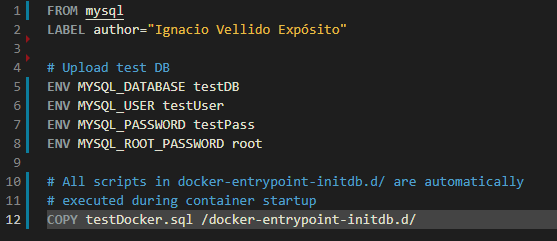
\includegraphics[width=.95\linewidth]{img/sgbd/s9.png}\caption{Dockerfile modificado.}\end{figure}

\begin{figure}[H]\center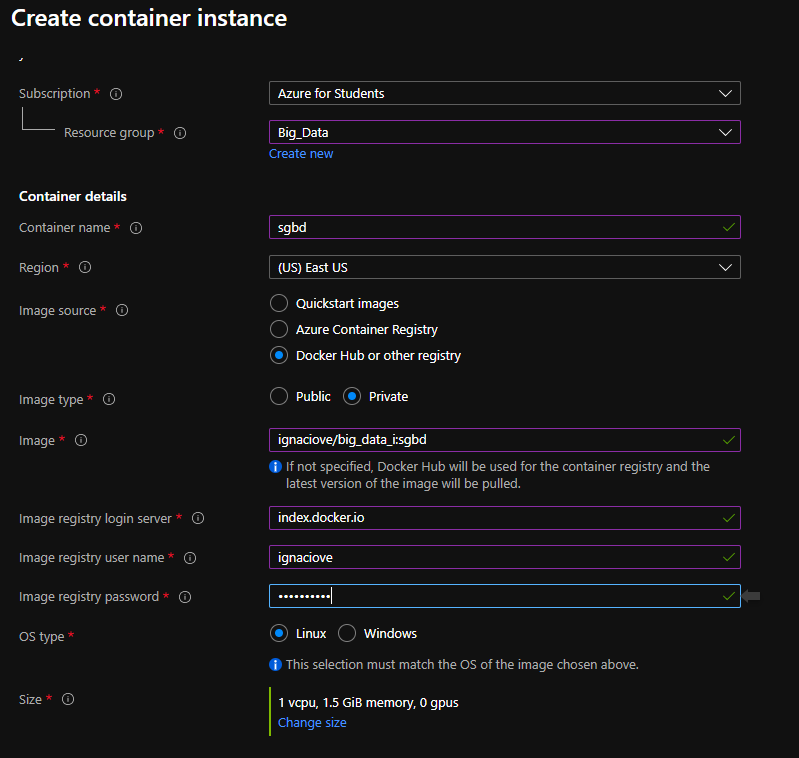
\includegraphics[width=.95\linewidth]{img/sgbd/s5.png}\caption{Creando contenedor.}\end{figure}

\begin{figure}[H]\center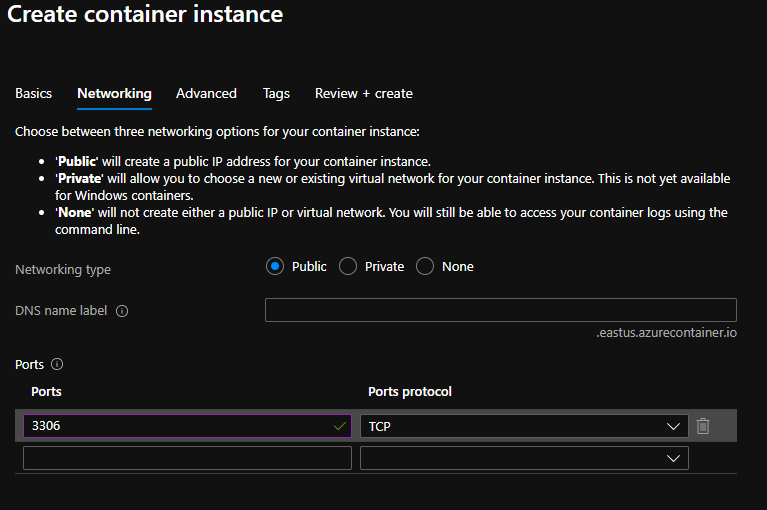
\includegraphics[width=.95\linewidth]{img/sgbd/s6.png}\caption{Indicando el puerto exportado.}\end{figure}

\begin{figure}[H]\center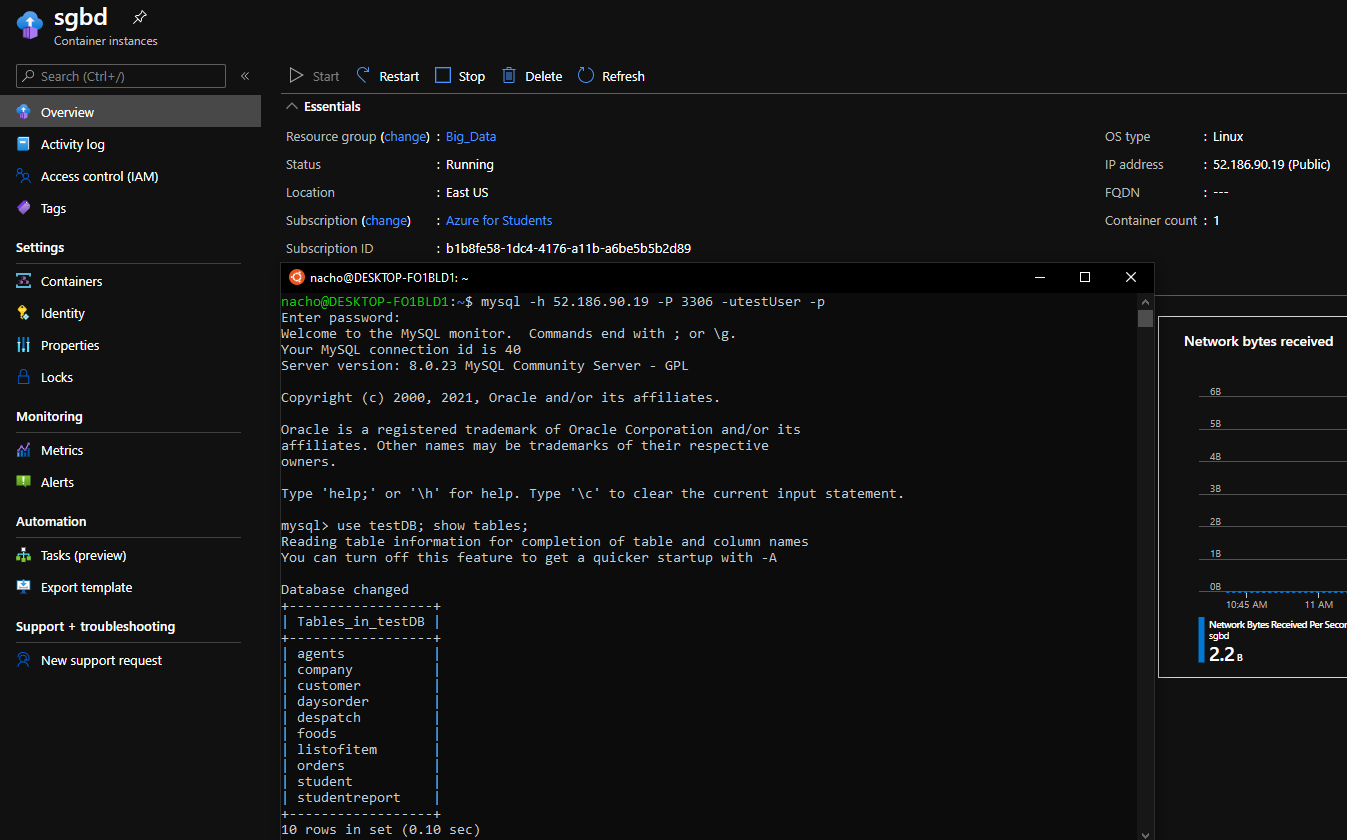
\includegraphics[width=.95\linewidth]{img/sgbd/s7.png}\caption{Accediendo a través de la IP pública.}\end{figure}

\begin{figure}[H]\center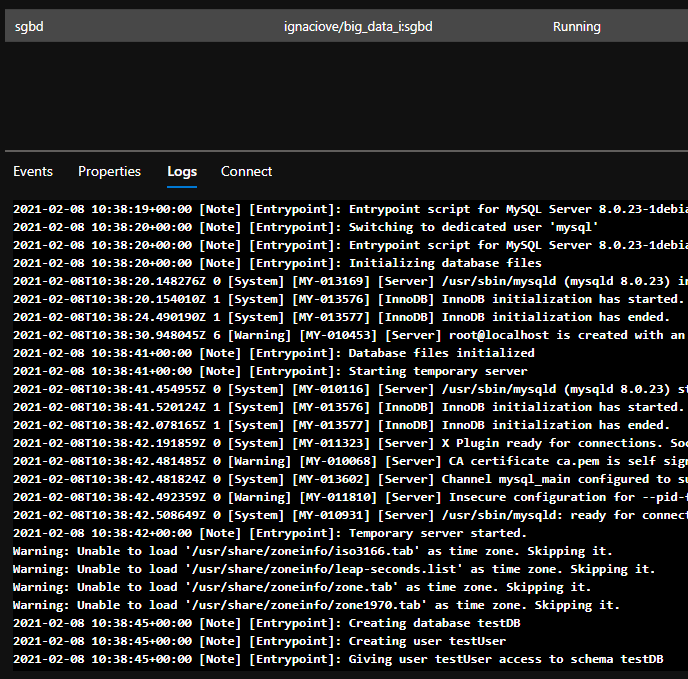
\includegraphics[width=.95\linewidth]{img/sgbd/s8.png}\caption{Logs del contenedor.}\end{figure}

\newpage

\subsection{Evaluación}

La evaluación únicamente se basa en poder acceder al usuario creado en el Dockerfile, corroborando la correcta inclusión de la base de datos de prueba.

\begin{figure}[H]\center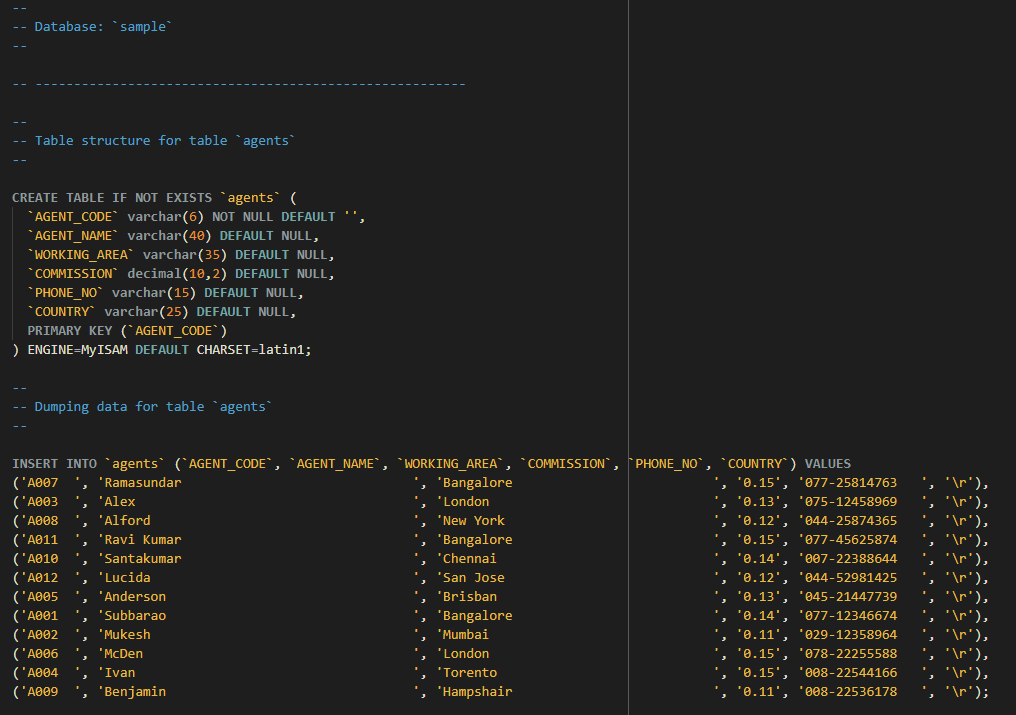
\includegraphics[width=.95\linewidth]{img/sgbd/s4.png}\caption{Fragmento de la base de datos insertada.}\end{figure}